\begin{figure}[H]
    \begin{center}
    \caption{Number of Ph.D. candidates by Program Rankings}
    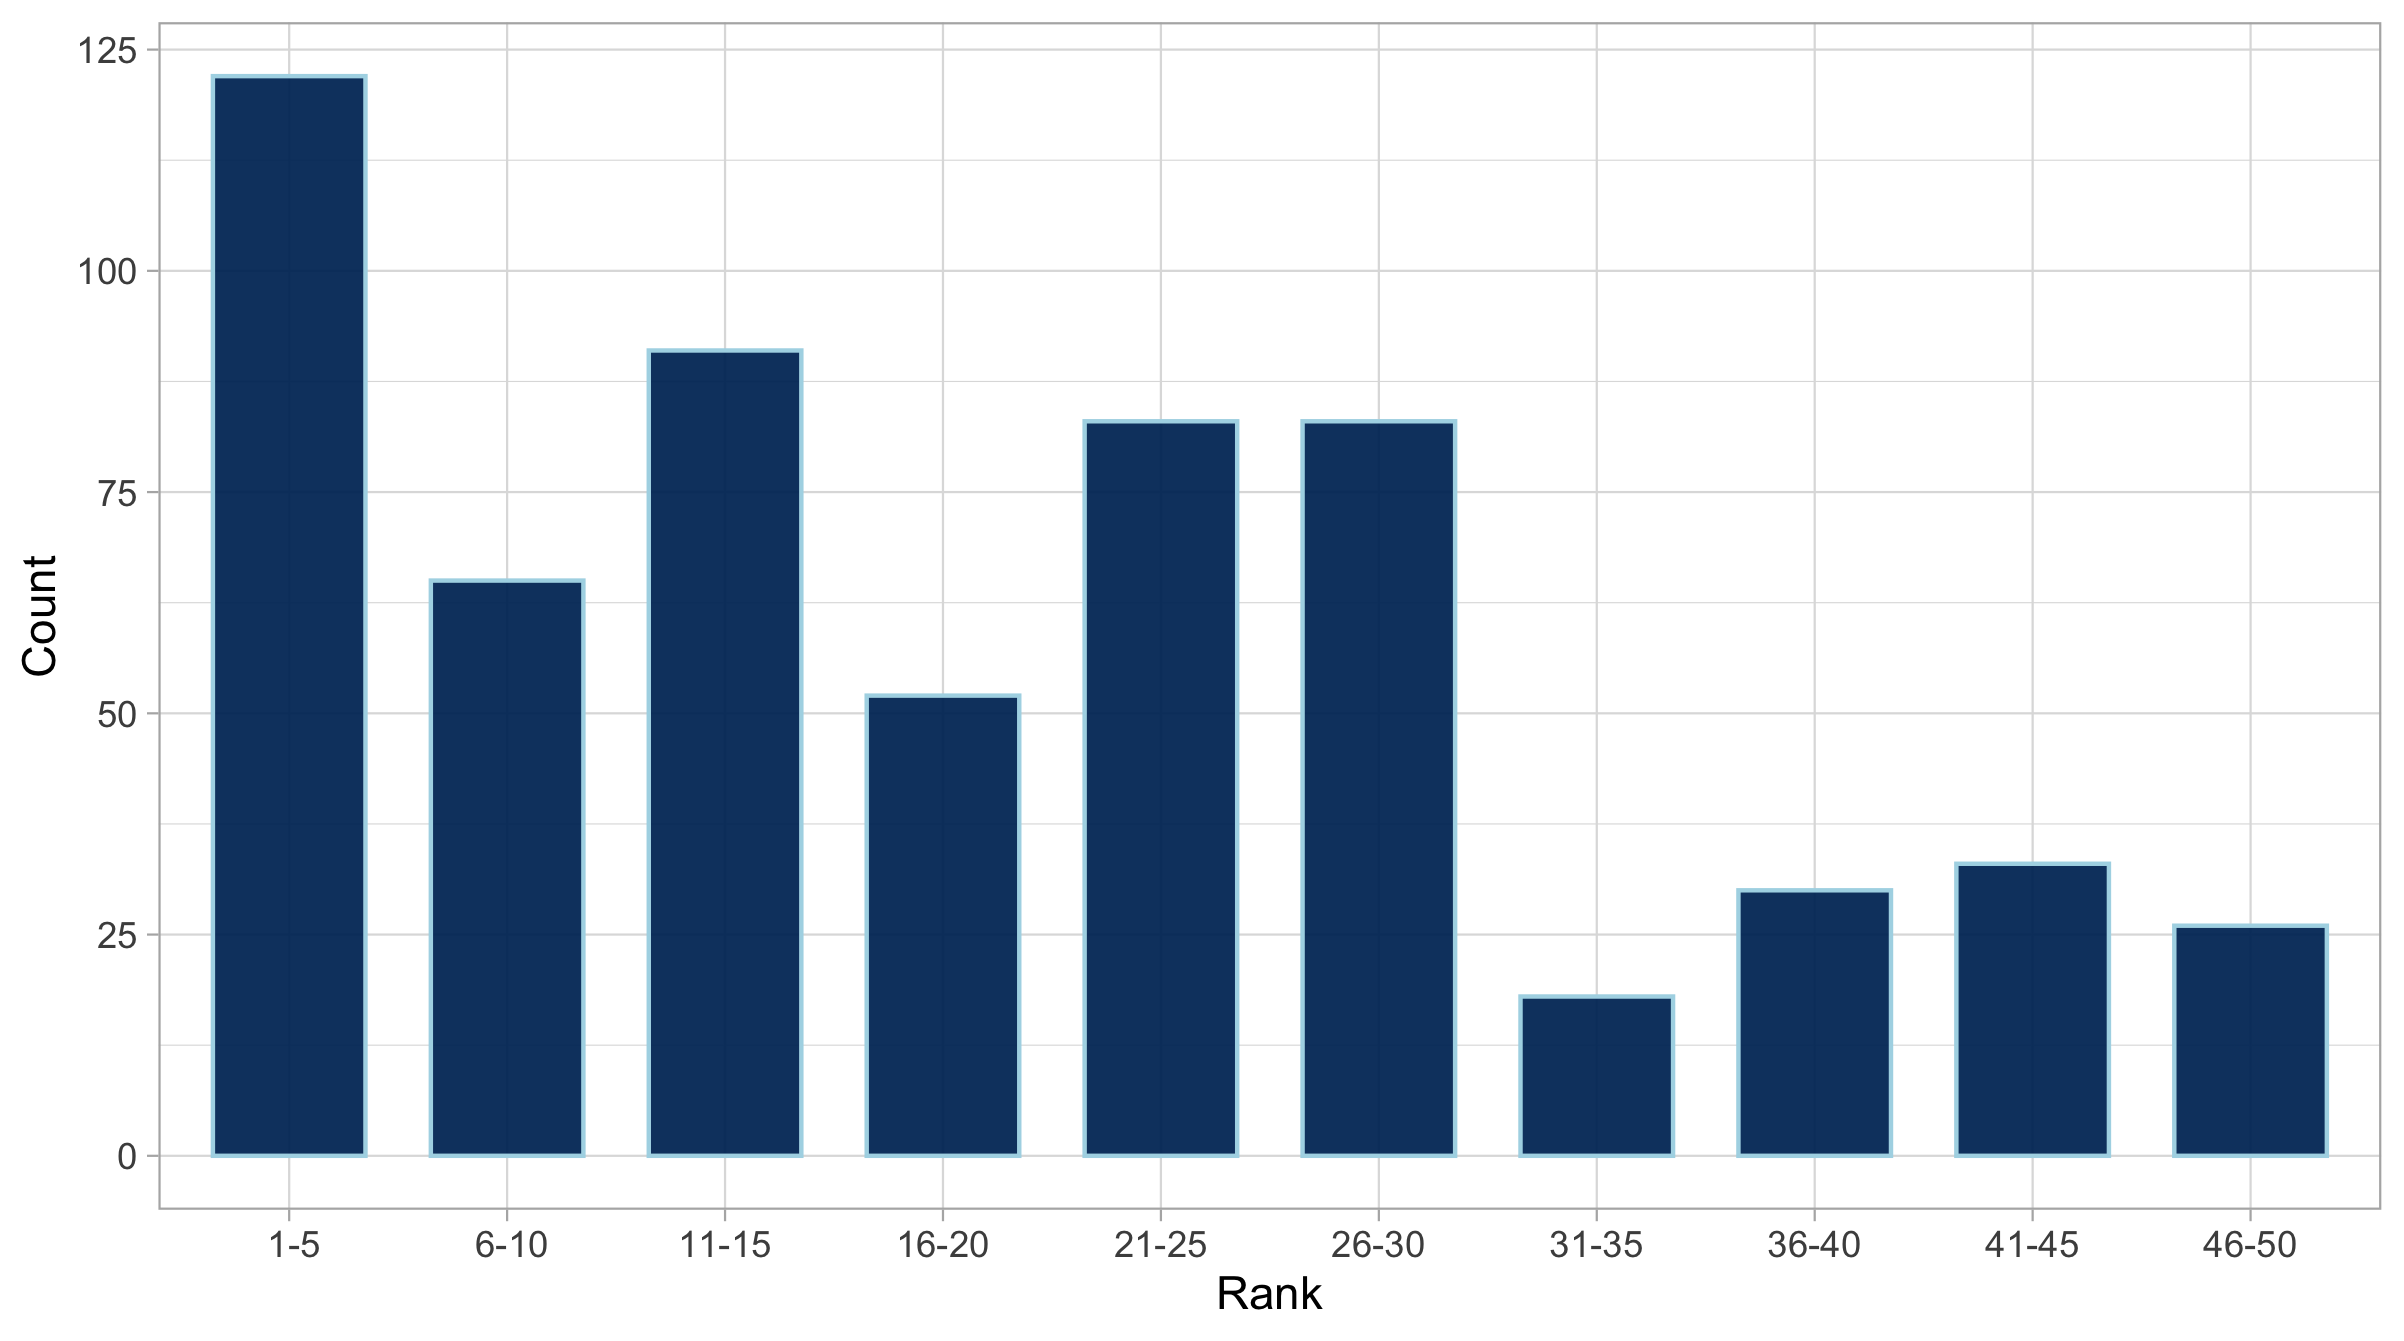
\includegraphics[width=140mm, scale=0.5]{fig/figure1.png}
    \end{center}
	\label{fig:figure1}
    \vspace{0.3cm}
    \begin{minipage}{0.95\textwidth} 
	{\footnotesize \textit{Note}: Figure presents the number of Ph.D. candidates by the program rankings. 50 Ph.D. programs are divided into 10 rank tiers. Note that there does not have to be 5 schools in each tier, for example, the tier 1 to 5 has 7 programs tied for first place.
	\par
	}
	\end{minipage}
\end{figure}
